% Technischer System- und Evaluationsbericht zum Masterprojekt (12 CP), LLNCS-Layout.
% Dokumentierter Umfang: bereinigter ReID-Kern auf main; Stand: 20.09.2026.
% Die explorative Vier-Video-Evaluation wurde mit zwölf Verarbeitungsläufen durchgeführt.
\documentclass[runningheads,a4paper]{llncs}

\usepackage[T1]{fontenc}
\usepackage[utf8]{inputenc}
\usepackage[english,ngerman]{babel}
\usepackage{graphicx}
\usepackage{amsmath}
\usepackage{booktabs}
\usepackage{tabularx}
\usepackage{xcolor}
\usepackage{xurl}
\usepackage{microtype}

\newcommand{\systemname}{Local Person Re-Identification MVP}
\newcommand{\todoentry}[1]{\textcolor{red!70!black}{[#1]}}
\begin{document}

\title{Entwicklung eines lokalen Prototyps zur Person-Wiedererkennung mit qualitätsbasierter Ausschnittsauswahl}
\titlerunning{Lokale Person-Re-Identifikation}

% TODO: Autorinnen und Autoren sowie Hochschulangaben ergänzen.
\author{\todoentry{Vorname Nachname}}
\authorrunning{\todoentry{Nachname}}
\institute{\todoentry{Hochschule für angewandte Wissenschaften}\\
\todoentry{Fakultät / Masterstudiengang / Modul}\\
\email{\todoentry{hochschul-email@example.org}}}

\maketitle

\begin{abstract}
Im Rahmen des Masterprojekts wurde ein lokal ausführbarer Prototyp zur Wiedererkennung von Personen in Videos und Kameraaufnahmen entwickelt. Er verbindet YOLO-basierte Detektion und kurzfristiges Tracking mit persistenten synthetischen Personenkennungen. Qualitätsgefilterte Ausschnitte werden durch OSNet codiert und zu gewichteten Profilen zusammengeführt. Eine Ähnlichkeitsprüfung vor Profilupdates soll falsche Aktualisierungen begrenzen. Der Projektbeitrag liegt in der technischen Integration dieser Verfahren und ihrer nachvollziehbaren Erprobung. Hierzu wurden zwei Personen in vier Videos mit drei festen Konfigurationen verarbeitet. Die zwölf Läufe dienen dem Vergleich der vollständigen OSNet-Pipeline mit Varianten ohne Qualitätsschwellen beziehungsweise Update-Schutz. Von sechs betrachteten Rückkehrereignissen wurden mit der Referenzkonfiguration und ohne Update-Schutz jeweils fünf korrekt erkannt. Ohne Qualitätsschwellen waren es drei. Im betrachteten Kreuzungsfenster traten drei korrekte Eigenkandidaten und keine Fremdkandidaten auf. Auf der verwendeten CPU erreichten die Varianten ungefähr 19 Frames pro Sekunde und damit bei 30-FPS-Videos keine Echtzeitverarbeitung. Diese Werte dokumentieren das Verhalten des Prototyps in den ausgewählten Projektszenarien; wegen des kleinen und szenarisch eng begrenzten Videobestands erlauben sie keine allgemeine Leistungsbewertung.
\keywords{Person ReID \and Computer Vision \and Tracking \and OSNet}
\end{abstract}

\section{Einleitung und Projektziel}
In den vergangenen Jahren haben Verfahren des maschinellen Sehens deutliche Fortschritte erzielt: Personen und Objekte lassen sich in Videodaten mit hoher Geschwindigkeit erkennen und über mehrere Frames hinweg verfolgen, zunehmend auch lokal und auf gängiger Consumer-Hardware statt auf spezialisierter oder serverseitiger Infrastruktur. Eine weiterhin relevante Herausforderung bleibt jedoch, Personen auch nach Unterbrechungen zuverlässig wiederzuerkennen -- genau hier setzt die vorliegende Arbeit an.

Eine Person im Video zu detektieren unterscheidet sich von der Aufgabe, eine Person zu re-identifizieren. Die Detektion erkennt die Anwesenheit einer Person und liefert ihre Position im Bild. Die Re-Identifikation vergleicht ihre visuellen Merkmale mit gespeicherten Personenprofilen und prüft, ob sie bereits zuvor beobachtet wurde oder ob es sich um eine neue Person handelt. Durch Tracking lassen sich beide Aufgaben verbinden, indem die detektierte Person über die Folge mehrerer Frames hinweg verfolgt wird und ihre Identität somit erhalten bleibt. Dabei können jedoch Unterbrechungen auftreten, etwa durch Verdeckung, Abwesenheit oder unzureichende Detektion. In solchen Fällen ist die Re-Identifikation erforderlich, um der Person nach ihrer Rückkehr die korrekte Identität zuzuordnen.

Nicht jeder detektierte Personenausschnitt eignet sich dabei gleich gut für den Profilabgleich. Ausschnitte können unscharf, zu klein, zu gering aufgelöst oder von ungünstiger Beleuchtung beeinflusst sein, was Personenzuordnungen erschwert oder Personenprofile verfälscht.

Anwendungsszenarien für Re-Identifikation sind etwa Bewegungsstudien in kontrollierten Innenräumen, bei denen Personen das Sichtfeld verlassen und später zurückkehren. Daraus ergibt sich die zentrale Fragestellung dieser Arbeit:
Wie lässt sich eine lokale Videoanalyse aufbauen, die Personen kontinuierlich verfolgt, bei einer Rückkehr zuverlässig wiedererkennt und dabei die Qualität ihrer gespeicherten Merkmale berücksichtigt?

Ziel des Masterprojekts ist die Erstellung und Konfiguration einer lokalen Re-Identifikations-Pipeline für Videos und Kameraaufnahmen. Das System vergibt dabei synthetische Personenkennungen, um nicht auf die tatsächliche Identität der Personen angewiesen zu sein.

Detektion, Tracking und Re-Identifikation sind einzeln etablierte Verfahren. Auch ihre Kombination ist keine neue Idee. StrongSORT ist ein Beispiel dafür~\cite{du2023strongsort}.
Das Ergebnis des Projekts ist die Integration dieser Verfahren zu einem lokalen Prototyp mit fester Qualitätsheuristik, gewichteter Profilbildung und Ähnlichkeitsschutz vor Profilupdates. Eine ereignisbasierte Erprobung beschreibt, wie sich diese Mechanismen in ausgewählten, kontrollierten Projektszenarien verhalten.

Vorgesehen ist ein kontrollierter Einzelplatzbetrieb mit zwei Personen, der auch bei einer direkt angeschlossenen Kamera in praktikabler Zeit nutzbar sein soll. Mehrkamerabetrieb, Gesichtserkennung und produktive Personenüberwachung liegen au{\ss}erhalb des Projektumfangs.


\section{Verfahren und Systementwurf}
\label{sec:design}

\subsection{Gesamtarchitektur}

Das System folgt dem Prinzip Tracking-by-Detection. Zunächst werden Personen in einem Frame detektiert und ihre Positionen durch Bounding Boxes beschrieben. Der Tracker verbindet diese Detektionen über mehrere Frames hinweg zu Spuren. Aus den Personen-Boxen werden anschlie{\ss}end Ausschnitte entnommen, deren Qualität geprüft wird. Für geeignete Ausschnitte werden visuelle Merkmalsvektoren berechnet, die mit gespeicherten Personenprofilen verglichen oder als neues Profil angelegt werden. Abbildung~\ref{fig:architecture} zeigt diese Verarbeitungskette.

Dabei unterscheidet die Anwendung zwei Kennungen: eine temporäre
Trackkennung, die zur aktuellen Spur gehört, und eine persistente
Personenkennung, die zu einem gespeicherten Profil gehört. Eine Person kann somit nach dem Verlust ihrer Spur eine neue Trackkennung erhalten, während ihre Personenkennung bei erfolgreichem Profilabgleich erhalten bleibt.

Ob eine Spur bereits eine Personenkennung besitzt, entscheidet über den weiteren Ablauf. Eine neue Spur durchläuft zunächst die Zuordnung zu einem Personenprofil (Abschnitt~\ref{sec:new-profile}). Eine bereits zugeordnete Spur hingegen erhält nur noch periodische, geschützte Profilupdates (Abschnitt~\ref{sec:profile-update}).
Detektion und Tracking, Merkmalsberechnung, Matching, Profilaktualisierung und Speicherung sind über getrennte Schnittstellen
angebunden, sodass sich einzelne Komponenten austauschen lassen, ohne die gesamte Verarbeitungskette zu verändern.

\begin{figure}[tbp]
\centering
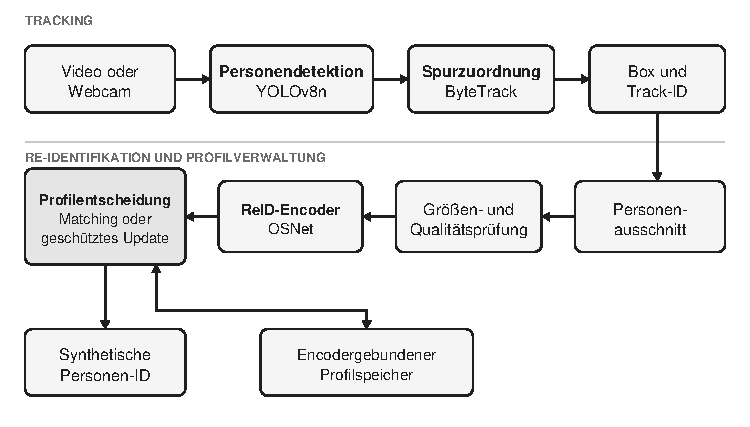
\includegraphics[width=\linewidth]{figures/systemarchitektur.pdf}
\caption{Verarbeitungskette des lokalen Prototyps. Qualitätsprüfung und Re-Identifikation erfolgen nach der Spurzuordnung und beeinflussen das Tracking nicht.}
\label{fig:architecture}
\end{figure}

\subsection{Personendetektion und Tracking}

Für die Personendetektion wird das COCO-vortrainierte Modell YOLOv8n verwendet~\cite{ultralytics-yolov8}. Es liefert Bounding Boxes und eine Detektionskonfidenz für die Klasse Person. Das System berücksichtigt nur diese Klasse, und Detektionen unterhalb der eingestellten Konfidenzschwelle werden verworfen, bevor sie an den Tracker übergeben werden. Die Referenzwerte stehen in Tabelle~\ref{tab:defaults}. Detektion und Tracking werden über Ultralytics eingebunden~\cite{ultralytics-track}.

ByteTrack ordnet die verbleibenden Detektionen anhand der Boxpositionen und der geschätzten Bewegung bestehenden Spuren zu~\cite{zhang2022bytetrack}. Seine Zuordnungsregeln bestimmen, ob eine Spur fortgeführt oder eine neue aufgebaut wird. Andere Tracker, etwa Deep SORT, verwenden gelernte Erscheinungsmerkmale bereits bei der Spurzuordnung~\cite{wojke2017deepsort}. In dieser Pipeline erfolgt der ReID-Profilabgleich dagegen erst nach dem Tracking, als eigener Verarbeitungsschritt. Verwendet wird ByteTrack aus Ultralytics 8.4.60 mit den in Tabelle~\ref{tab:defaults} dokumentierten Einstellungen.

\subsection{Zuordnung eines neuen Personenprofils}
\label{sec:new-profile}
Solange eine Spur noch keine Personenkennung besitzt, wird sie als Kandidat für ein neues Profil betrachtet. Die Personenausschnitte werden dabei aus dem ursprünglichen Frame entnommen, bevor Boxen oder Trackkennungen eingezeichnet werden. Boxen ohne Trackkennung tragen nicht zu einem Personenprofil bei. Das System prüft zunächst für jeden Ausschnitt der Spur, ob er geometrisch gültig ist und die Mindestgrö{\ss}e erfüllt.

Anschlie{\ss}end ermittelt das System Schärfe, Helligkeit, Grö{\ss}e, Seitenverhältnis, Randkontakt und Detektionskonfidenz. Daraus wird ein gewichteter Qualitätswert $Q$ zwischen null und eins berechnet. Schärfe und Grö{\ss}e erhalten dabei das höchste Gewicht.

Ein Initialkandidat muss zusätzlich zur Gesamtqualitätsschwelle $Q\geq q_{\mathrm{init}}$ zwei eigene Mindestgrenzen erfüllen, die unabhängig vom Gesamtwert $Q$ gelten: eine für die Schärfe $s_{\mathrm{init}}$ und eine für die Bewertung des Seitenverhältnisses $a_{\mathrm{init}}$. Berührt die ursprüngliche Bounding Box einen Bildrand, verschärft sich die Schärfegrenze zusätzlich auf $s_{\mathrm{Rand}}$, während gleichzeitig der Randteilwert $R$ in der Berechnung von $Q$ auf $\rho_{\mathrm{Rand}}$ sinkt. Ein randberührender, unscharfer Ausschnitt wird so über zwei Wege erfasst: einmal durch den niedrigeren Gesamtwert $Q$, einmal durch die eigene Schärfegrenze. Eine gute Grö{\ss}e oder Helligkeit kann einen deutlich unscharfen oder untypisch breiten Ausschnitt dadurch nicht allein über $Q$ ausgleichen. Die konkreten Parameterwerte stehen in Tabelle~\ref{tab:pilot-grid}, die Berechnung beschreibt Anhang~\ref{app:profile-details}.

Erfüllt ein Ausschnitt alle für die jeweilige Konfiguration geltenden Grenzen, berechnet OSNet-x1.0 ein 512-dimensionales Embedding~\cite{zhou2019osnet}. Die verwendeten Modellgewichte stammen aus dem Training auf MSMT17~\cite{torchreid-modelzoo}. Eigenes Training oder Fine-Tuning findet nicht statt.

Vor der ersten Profilentscheidung sammelt das System die ersten fünf akzeptierten Embeddings derselben Spur in einem Initialpuffer. Jeder geeignete Frame kann einen Kandidaten beitragen, abgelehnte Ausschnitte werden dabei nicht aufgenommen. Erreicht eine Spur bis zum Videoende keine fünf Kandidaten, bleibt sie ohne Personenkennung.

Um vermischte Ausschnitte bei einer Kreuzung zu begrenzen, prüft das System vor der Merkmalsberechnung die Überdeckung gleichzeitig erkannter Personen. Überschreitet die Schnittfläche relativ zur kleineren Bounding Box den konfigurierten Grenzwert, nimmt das System keinen Initialkandidaten auf und leert den bestehenden Initialpuffer der betroffenen unbekannten Spur. Während einer anschlie{\ss}enden kurzen Abkühlphase sammelt es ebenfalls keine Kandidaten. Dadurch gehen Ausschnitte vor und nach einer erkannten Kreuzung nicht gemeinsam in die erste Profilentscheidung ein. Die genaue Berechnung steht in Anhang~\ref{app:profile-details}.

Sobald fünf Ausschnitte angenommen wurden, werden ihre normalisierten Embeddings $z_i$ qualitätsgewichtet zusammengeführt:
\begin{equation}
\bar z=\operatorname{norm}\left(\frac{\sum_i w_i z_i}{\sum_i w_i}\right),
\qquad w_i=\max(Q_i,0{,}05).
\label{eq:fusion}
\end{equation}
Das feste Mindestgewicht $0{,}05$ sorgt dafür, dass auch bei deaktivierten Qualitätsschwellen jeder Beitrag zählt.

Gegen dieses zusammengeführte Embedding vergleicht das System alle zulässigen gespeicherten Profile mittels
Cosine Similarity. Für zwei normalisierte Vektoren $z_q$ und $z_p$ entspricht dies dem Skalarprodukt:
\begin{equation}
s(z_q,z_p)=z_q^\top z_p.
\label{eq:cosine}
\end{equation}
Bereits im aktuellen Frame sichtbare Personenkennungen schlie{\ss}t das System dabei von der Auswahl aus, um Doppelzuweisungen zu vermeiden. Erreicht das ähnlichste Profil den Matching-Schwellwert $\tau_{\mathrm{match}}$, ordnet das System seine Personenkennung der Spur zu. Andernfalls legt es ein neues Profil mit einer neuen Personenkennung an und ordnet es der Spur zu. Ein zusätzlicher Mindestabstand zum zweitbesten Profil wird dabei nicht geprüft. Neben dem Ergebnis protokolliert das System auch das ähnlichste geprüfte Profil, seinen Score und den Ablehnungsgrund. So bleibt ein knapp verfehlter Profilabgleich nachträglich nachvollziehbar.

Im ersten Fall prüft das System das zusammengeführte Embedding zusätzlich gegen die Update-Ähnlichkeitsschwelle $\tau_{\mathrm{upd}}$ aus Abschnitt~\ref{sec:profile-update}, bevor es in das bestehende Profil einflie{\ss}t. Eine wiedergefundene Person durchläuft damit denselben Update-Schutz wie ein reguläres Update. Wird diese Schwelle nicht erreicht, bleibt die Personenkennung zugeordnet, das Profil selbst aber unverändert.

\subsection{Aktualisierung eines zugeordneten Profils}
\label{sec:profile-update}

Sobald eine Spur eine Personenkennung besitzt, wird die Suche nach einem Profil abgeschlossen. In der verwendeten Referenzkonfiguration wird alle fünf Frames ein Profilupdate mit dem Personenausschnitt der Spur aus genau diesem Frame versucht.

Für ein Update muss der Ausschnitt die geometrischen Mindestanforderungen erfüllen. Sein Qualitätswert $Q$ wird dabei wie in Abschnitt~\ref{sec:new-profile} berechnet und muss $Q\geq q_{\mathrm{upd}}$ erfüllen. Die zusätzlichen Initialgrenzen für Schärfe und Seitenverhältnis gelten nicht für eine bereits zugeordnete Spur. Überlappung und Abkühlphase sperren dagegen auch reguläre Updates. Dadurch kann bei Updates ein schwacher Schärfeteilwert durch andere gute Teilwerte kompensiert werden. Die höhere Gesamtqualitätsschwelle begrenzt dies, stellt aber keine eigene Schärfegarantie dar.
Ebenfalls muss das Embedding laut Gleichung~\ref{eq:cosine} mindestens die Update-Ähnlichkeitsschwelle $\tau_{\mathrm{upd}}$ zum aktuell zugeordneten Profil erreichen. Scheitert eine der geometrischen, qualitativen, überdeckungsbezogenen oder ähnkeitsbezogenen Prüfungen, bleibt das Profil unverändert. Die Personenkennung der Spur bleibt weiterhin erhalten.

Dieser Schutz korrigiert also keine falsche Profilzuordnung, sondern verhindert nur, dass ein zweifelhafter Ausschnitt ein bestehendes Profil verfälscht. Eine einmal zugeordnete Spur wird nicht erneut gegen alle Profile geprüft. Ein Track-ID-Wechsel kann daher eine falsche Personenkennung an der Spur belassen, und ein fälschlich angelegtes Doppelprofil wird nicht automatisch zusammengeführt. Der Schutz kann au{\ss}erdem dazu führen, dass korrekte neue Ansichten einer Person nicht für ein Profilupdate berücksichtigt werden.

Wird ein Update angenommen, ergänzt das System das bestehende Profil, statt dessen Embedding zu ersetzen. Im Profil gespeichert sind die gewichtete Embeddingsumme $E$ und die Gewichtssumme $W$. Für ein neues Embedding $z$ mit Gewicht $w=\max(Q,0{,}05)$ gilt
\begin{equation}
E_{\mathrm{neu}}=E+wz,\qquad W_{\mathrm{neu}}=W+w,\qquad
p_{\mathrm{neu}}=\operatorname{norm}(E_{\mathrm{neu}}/W_{\mathrm{neu}}).
\label{eq:profile-update}
\end{equation}
Die fünf Initialbeobachtungen bleiben damit im Profil erhalten. Bei einer Wiedererkennung wird der neue Fünferblock gemeinsam ergänzt, sofern die Update-Ähnlichkeitsschwelle erfüllt ist. Jedes weitere angenommene Update erweitert das Profil, statt die bisherigen Beobachtungen zu ersetzen.

\subsection{Profilbestände und Modellwechsel}
Personenprofile werden lokal gespeichert und beim Ende einer Videoverarbeitung oder eines Prozesses nicht automatisch gelöscht. Bei Verwendung eines gemeinsamen Profilbestands können die gespeicherten Profile auch in späteren Videos für die Wiedererkennung verwendet werden. Der Trackerzustand gilt dagegen nur für die jeweilige Videoverarbeitung. Die synthetischen Kennungen anonymisieren die gespeicherten Embeddings und Schnappschüsse nicht; sie stellen lediglich eine Pseudonymisierung dar. Eine Löschung erfordert das Entfernen des betreffenden lokalen Profilbestands und der zugehörigen Ausgabedateien.

Jede Encoder-Konfiguration erhält einen eigenen Profilbestand. Die Trennung berücksichtigt Modellarchitektur, Modellgewichte und Vorverarbeitung, da verschiedene Encoder auch bei gleicher Vektordimension unterschiedliche Merkmalsräume erzeugen können. Bei einem Wechsel zu einer früheren Encoder-Konfiguration kann deren bisheriger Bestand wiederverwendet werden.

Zudem wird ein isolierter Lauf mit neuem Profilbestand ermöglicht, ohne frühere Bestände zu löschen. Welche Aufnahmen innerhalb der Erprobung einen Bestand teilen und welche getrennt verarbeitet werden, beschreibt der Testaufbau in Abschnitt~\ref{sec:reference}.

\section{Explorative Erprobung}
\label{sec:evaluation}
% TODO: Die zwölf Läufe nach Entfernung des Initialkandidatenabstands neu erzeugen
% und Ergebniswerte, Laufzeiten sowie Tabellen vor der Abgabe aktualisieren.

Die Erprobung dient dazu, das Verhalten des entwickelten Prototyps anhand konkreter Fälle nachvollziehbar zu dokumentieren. Betrachtet wird, ob die Pipeline Personen nach einer Rückkehr wiedererkennt, wie sie sich mit und ohne Qualitätsschwellen verhält und welche Updates der Ähnlichkeitsschutz in einem ausgewählten Kreuzungsszenario zulässt. Ergänzend wird die Verarbeitungsgeschwindigkeit gemessen. Aufgrund des kleinen Testumfangs werden daraus keine allgemeinen Wirksamkeits- oder Zuverlässigkeitsaussagen abgeleitet.

\subsection{Testaufbau und Referenzdaten}
\label{sec:reference}

Zwei Personen nehmen mit dokumentiertem Einverständnis an vier Eigenaufnahmen in einem kontrollierten Innenraum teil. Die Aufnahmen wurden mit einer Smartphone-Kamera erstellt und lagen für die Auswertung als MP4-Dateien mit einer Auflösung von $1024\times576$ Pixeln, ungefähr 30 Frames pro Sekunde und Dauern zwischen 27,7 und 39,9 Sekunden vor. Das genaue Gerätemodell wurde nicht protokolliert.

Für jedes Testszenario aus Tabelle~\ref{tab:evaluation-groups} liegt eine Aufnahme vor. Jede der vier Sequenzen wird mit drei Konfigurationen verarbeitet, sodass der projektinterne Vergleich zwölf Verarbeitungsläufe umfasst.
\begin{table}[tbp]
\caption{Vier Testszenarien mit jeweils einer Videoaufnahme.}
\label{tab:evaluation-groups}
\centering
\small
\begin{tabularx}{\linewidth}{@{}lp{0.29\linewidth}X@{}}
\toprule
Gruppe & Szenario & Schwerpunkt \\
\midrule
G1 & Freie Sicht & Mehrere Personen, Bewegung und unbekannter Eintritt. \\
G2 & Verlassen und Rückkehr & Wiedererkennung nach einer Unterbrechung der Spur. \\
G3 & Ähnliche Kleidung & Unterscheidung ähnlich gekleideter Personen bei einer Rückkehr. \\
G4 & Kreuzung / Verdeckung & Profilzuordnungen und -updates an kritischen Übergängen. \\
\bottomrule
\end{tabularx}
\end{table}
In G1 befindet sich zunächst eine Person im Bild, bevor eine zweite Person hinzukommt. G2 enthält gut unterscheidbare Kleidung sowie drei auswertbare Rückkehrereignisse. G3 enthält zwei schwarz gekleidete Personen und ebenfalls drei Rückkehrereignisse. In G4 kreuzen und verdecken sich beide Personen; danach entstehen zwei neue Spuren, deren erneute Profilzuordnung bewertet wird. Registrierung und spätere Ereignisse liegen jeweils innerhalb desselben Videos. Eine Konfiguration behält ihren Profilbestand über das betreffende Video, beginnt für das nächste Video jedoch wieder mit einer leeren Datenbank.

Die Kleidung ist dabei kontrolliert: In G1 und G2 tragen die Personen gut unterscheidbare Kleidung, während G3 gezielt den Fall ähnlicher Kleidung untersucht.

Für G4 wird um die zentrale Kreuzung bei Frame 316 ein Übergangsfenster von Frame 301 bis 391 verwendet. Dies entspricht ungefähr 0,5 Sekunden vor bis 2,5 Sekunden nach dem Übergang. In diesem Fenster werden die protokollierten Profilupdates geprüft.

Die Referenzannotation erfasst die beteiligte Person, den Zeitpunkt und die Sichtbarkeit bei Registrierung, Eintritt, Austritt und Rückkehr sowie in den ausgewählten G4-Fenstern. Eine vollständige Annotation sämtlicher Bounding Boxes erfolgt nicht. Die Erprobung ist damit ein projektspezifischer Funktionstest und kein vollständiger Detektions- oder Trackingbenchmark.

Ausschlüsse wegen uneindeutiger Sichtbarkeit oder einer Beobachtungsdauer von weniger als zwei Sekunden werden anhand der Referenzaufnahme festgelegt. Fehlende Detektionen, verlorene Spuren, abgelehnte Ausschnitte und fehlgeschlagene Registrierungen bleiben dagegen als Systemfehler in der Auswertung. Ein weiterer Eintritt in G2 wird ausgeschlossen, weil das Video vor Ablauf des vollständigen Zwei-Sekunden-Fensters endet und zunächst nur eine randberührende Teilansicht sichtbar ist. Die übrigen Ereignisse wurden anhand von Originalvideo, annotiertem Video und Frameprotokoll manuell zugeordnet.

Jede Konfiguration beginnt pro Testeinheit mit einem frischen Tracker und einem leeren Profilbestand. Profile bleiben nur innerhalb der jeweiligen Sequenz beziehungsweise des zusammengehörigen Registrierungs-/Rückkehrpaars erhalten. Varianten und getrennte Testeinheiten beeinflussen sich dadurch nicht gegenseitig.

\subsection{Testkonfigurationen und Pilotabstimmung}
\label{sec:calibration}

Matching-Schwelle, Update-Ähnlichkeit sowie Kandidaten- und Updatequalität wurden in vorausgehenden explorativen Läufen schrittweise geprüft. Hierfür wurden separate Pilotvideos desselben Szenariotyps verwendet, auf denen andere Personen als in den vier Testvideos zu sehen waren. Die Pilotvideos und die vier ausgewerteten Aufnahmen überschneiden sich somit weder auf Video- noch auf Personenebene. Das daraus abgeleitete Preset \texttt{best-calibrated} wurde anschlie{\ss}end für alle zwölf Auswertungsläufe unverändert verwendet. Das Suchraster steht in Anhang~\ref{app:pilot-details}.

Für B0 wurden eine Matching-Schwelle von 0,75, eine Kandidatenqualität von 0,55, eine Updatequalität von 0,65 und eine Update-Ähnlichkeit von 0,75 verwendet. Die im Pilotversuch festgelegten zusätzlichen Initialgrenzen und der Randwert stehen in Tabelle~\ref{tab:pilot-grid}.

Die in Tabelle~\ref{tab:defaults} aufgeführten Rahmenparameter blieben während der Pilotabstimmung und in den zwölf Auswertungsläufen konstant.

\begin{table}[tbp]
\caption{Konstante Rahmenparameter der explorativen Erprobung.}
\label{tab:defaults}
\centering
\small
\begin{tabularx}{\linewidth}{@{}Xl@{}}
\toprule
Parameter & Wert \\
\midrule
Detektionsmodell / Tracker & YOLOv8n / ByteTrack (Ultralytics 8.4.60) \\
Detektionskonfidenz & 0,35 \\
Eingangsgrö{\ss}e für YOLO & 640 Pixel \\
ByteTrack: high / low / new / match & 0,25 / 0,10 / 0,25 / 0,80 \\
ByteTrack: Puffer / Score-Fusion & 30 Frames / aktiv \\
Updateintervall & 5 Frames \\
Initialbeobachtungen & 5 \\
Minimale Cropgrö{\ss}e & $30\times80$ Pixel \\
Crop-Padding & 0,05 \\
Überdeckungsgrenze / Abkühlphase & 0,15 / 11 Frames \\
\bottomrule
\end{tabularx}
\end{table}

Updateintervall, Grenzwert für Überdeckung und Abkühlphase wurden während der technischen Entwicklung als feste Heuristiken gewählt. Sie waren keine Variablen des begrenzten Schwellenrasters in Anhang~\ref{app:pilot-details}. Die Angaben in Frames beziehen sich auf die Eingangssequenz. Bei den Testvideos entsprechen fünf Frames ungefähr 0,17 Sekunden und der ByteTrack-Puffer von 30 Frames ungefähr einer Sekunde.

Tabelle~\ref{tab:variants} zeigt die drei für die Auswertung festgelegten Konfigurationen.

\begin{table}[tbp]
\caption{Drei feste Konfigurationen des Komponentenvergleichs.}
\label{tab:variants}
\centering
\small
\begin{tabularx}{\linewidth}{@{}Xccc@{}}
\toprule
Variante & Matching & Qualität & Update-Schutz \\
\midrule
B0: vollständig & 0,75 & 0,55 / 0,65 & 0,75 \\
A2: ohne Qualitätsschwellen & 0,75 & 0 / 0 & 0,75 \\
A3: ohne Update-Schutz & 0,75 & 0,55 / 0,65 & aus ($-1$) \\
\bottomrule
\end{tabularx}
\end{table}

B0 bildet die vollständige OSNet-Referenz. A2 setzt die Gesamtqualitätsschwellen für Initialisierung und Update sowie die drei zusätzlichen Initialgrenzen für allgemeine Schärfe, Schärfe bei Randkontakt und Seitenverhältnis auf null. Mindestgrö{\ss}e, Berechnung und Gewichtung mit $Q$, Überlappungsschutz und Anzahl der Initialbeobachtungen bleiben unverändert. A3 deaktiviert ausschlie{\ss}lich die Update-Ähnlichkeitsschwelle.

\subsection{Auswertungskriterien}
\label{sec:metrics}

\paragraph{Wiedererkennung.}
Bei einer Rückkehr einer Person ist die erste ausgegebene Personenkennung innerhalb von zwei Sekunden nach dem ersten wieder sichtbaren Frame ma{\ss}geblich. Sie wird einer von vier Kategorien zugeordnet: richtige frühere Kennung, falsche bestehende Kennung, neue Kennung oder keine Entscheidung. Eine spätere Korrektur zählt nicht rückwirkend als rechtzeitiger Erfolg.

Die Rückkehr-Erfolgsrate lautet:
\begin{equation}
R_{\mathrm{return}}=
\frac{\text{rechtzeitig korrekt wiedererkannte Rückkehrereignisse}}
{\text{alle auswertbaren Rückkehrereignisse}}.
\label{eq:reentry}
\end{equation}

Fehlregistrierungen und fehlende Entscheidungen gehen als Misserfolge in den Nenner ein. Ergänzend wird berichtet, bei wie vielen Rückkehrereignissen tatsächlich eine neue Spur vorlag. Für einen unbekannten Eintritt gilt eine neue, bislang nicht belegte Personenkennung als korrekt. Zusätzlich wird die Videozeit vom ersten sichtbaren Frame bis zur korrekten Kennung ausgewertet.

\paragraph{Profilupdates.}
In den vorab festgelegten G4-Fenstern werden alle Updatekandidaten geprüft, die die geometrischen und qualitativen Anforderungen erfüllen und deshalb die Update-Ähnlichkeitsprüfung erreichen. Anhand des verwendeten Ausschnitts wird bestimmt, ob er den Eigentümer des zugeordneten Profils oder eine andere Person zeigt. Zusammen mit der Systementscheidung entstehen vier Fälle: korrekt angenommene Eigenkandidaten, fälschlich abgelehnte Eigenkandidaten, falsch angenommene Fremdkandidaten und korrekt abgelehnte Fremdkandidaten.

Berichtet werden der Anteil korrekt angenommener Eigenkandidaten an allen auswertbaren Eigenkandidaten und der Anteil falsch angenommener Fremdkandidaten an allen auswertbaren Fremdkandidaten. Die zugrunde liegenden vier Fallzahlen werden zusätzlich angegeben. Uneindeutige Ausschnitte werden separat gezählt und aus den Nennern ausgeschlossen. Ist ein Nenner leer, wird der betreffende Anteil als nicht definiert ausgewiesen.

\paragraph{Verarbeitungsgeschwindigkeit.}
Die Geschwindigkeit wird über den Real-Time-Faktor als Verhältnis von Verarbeitungsdauer zu Videodauer angegeben. Die gemessene Dauer umfasst Einlesen, Inferenz, Speicherung und Ergebnisausgabe. Die Modellladezeit wird separat betrachtet. Berichtet wird die zusammengefasste Verarbeitung der vier Videos je Konfiguration auf derselben CPU und ohne interaktive Vorschau. Die Läufe erfolgten unter Windows~11 mit Python~3.13.1 und PyTorch~2.12.0 im CPU-Betrieb; CUDA war nicht verfügbar. Zusätzliche technische Wiederholungen wurden nicht durchgeführt.

\subsection{Beobachtete Ergebnisse und Komponentenvergleich}

Die drei Konfigurationen werden auf denselben Testsequenzen gegenübergestellt. Berichtet werden die beobachteten Ereigniszähler mit den jeweiligen Nennern. Die Rückkehrergebnisse werden zusätzlich für G2 und G3 getrennt ausgewiesen. Für die Zeit bis zur korrekten Personenkennung wird der Median über alle erfolgreichen Rückkehrereignisse angegeben. Die Kennzahlen beschreiben ausschlie{\ss}lich diesen Testbestand; einzelne Frames werden nicht als unabhängige Stichproben behandelt.

Tabelle~\ref{tab:results-reid} enthält die zentralen Ergebnisse. \emph{n.\,d.} bezeichnet einen rechnerisch nicht definierten Anteil. Alle Anteile werden zusammen mit Zähler und Nenner angegeben.
\begin{table}[tbp]
\caption{Zentrale Ergebnisse der drei Konfigurationen auf demselben Ereignisbestand.}
\label{tab:results-reid}
\centering
\small
\begin{tabularx}{\linewidth}{@{}Xrrr@{}}
\toprule
Kenngrö{\ss}e & B0 & A2 & A3 \\
\midrule
Rückkehr korrekt / gesamt & 5/6 (83,3\,\%) & 3/6 (50,0\,\%) & 5/6 (83,3\,\%) \\
G2: Rückkehr korrekt / gesamt & 3/3 & 2/3 & 3/3 \\
G3: Rückkehr korrekt / gesamt & 2/3 & 1/3 & 2/3 \\
G1: Eintritt rechtzeitig neue ID & 0/1 & 1/1 & 0/1 \\
G4: Neuzuweisung rechtzeitig korrekt & 0/2 & 1/2 & 1/2 \\
Falsche bestehende ID bei Rückkehr & 0/6 & 0/6 & 0/6 \\
Neue ID bei registrierter Rückkehr & 1/6 & 3/6 & 1/6 \\
Eigenkandidaten angenommen / gesamt & 0/3 & 0/3 & 3/3 \\
Fremdkandidaten angenommen / gesamt & n.\,d. & n.\,d. & n.\,d. \\
Zeit bis korrekter Rückkehr-ID, Median in s & 1,13 & 1,13 & 1,13 \\
Verarbeitung in FPS & 19,11 & 18,80 & 19,02 \\
Real-Time-Faktor & 1,569 & 1,594 & 1,576 \\
\bottomrule
\end{tabularx}
\end{table}

\section{Auswertung und Grenzen}
\label{sec:discussion}

\subsection{Einordnung der Beobachtungen}

Mit B0 wurden fünf von sechs Rückkehrereignissen korrekt erkannt, davon drei von drei in G2 und zwei von drei bei ähnlicher schwarzer Kleidung in G3. Der einzige Fehler war eine neue Kennung statt der Wiederverwendung des vorhandenen Profils. A2 erreichte ohne Qualitätsschwellen drei von sechs korrekte Rückkehrentscheidungen, vergab aber beim G1-Eintritt und einer G4-Neuzuweisung schneller eine Kennung. Diese Einzelfälle zeigen einen möglichen Zielkonflikt zwischen früher Entscheidung und stabiler Profilwiederverwendung; der Median erfolgreicher Rückkehrentscheidungen betrug in allen Varianten 1,13 Sekunden.

Im G4-Fenster erreichten drei Eigen- und keine Fremdkandidaten die Update-Entscheidung. B0 und A2 lehnten die Eigenkandidaten bei Ähnlichkeiten von 0,55 bis 0,64 ab; A3 nahm sie an und erkannte danach eine von zwei neu entstandenen Spuren rechtzeitig wieder. Ein Schutzvorteil gegen Profilverunreinigung ist ohne Fremdkandidaten nicht belegt, während in diesem Einzelfall drei korrekte Updates verworfen wurden. Die gleiche Rückkehrquote von B0 und A3 erlaubt dennoch keinen allgemeinen Vorteil des deaktivierten Schutzes.

Über jeweils 4.165 Frames erreichten B0 19,11, A2 18,80 und A3 19,02 FPS. Die Verarbeitung benötigte damit rund 57 bis 59\,\% länger als die Videodauer; Echtzeit für 30-FPS-Videos wurde nicht erreicht. Die kleinen Unterschiede wurden nicht durch Wiederholungsläufe abgesichert.

\subsection{Grenzen der Aussagekraft}

Die Wiedererkennung stützt sich auf visuelle Erscheinungsmerkmale und ein einziges Profil je Kennung. Ähnliche Kleidung, Perspektivwechsel, Verdeckungen und kleine Ausschnitte können daher die Unterscheidbarkeit verringern. Die Zuordnung einer aktiven Spur ist zudem nicht reversibel: Nach einem Track-ID-Wechsel wird sie nicht erneut gegen alle Profile geprüft, und getrennte Doppelprofile werden nicht zusammengeführt. Der Update-Schutz kann eine Profiländerung verhindern, aber keine falsche Kennung korrigieren. Beim initialen Matching fehlt au{\ss}erdem ein Mindestabstand zum zweitbesten Profil.

Für Updates gelten keine eigenen harten Schärfe- oder Seitenverhältnisgrenzen; schwache Teilwerte können durch andere Bestandteile von $Q$ kompensiert werden. Zugleich wurden korrekte Einzelansichten abgelehnt, obwohl ein fusionierter Initialvektor derselben Person den gleichen Ähnlichkeitsschwellwert erreichte. Ob ein Schärfefilter, eine niedrigere Update-Schwelle oder mehrere ansichtsspezifische Profile geeigneter wären, bleibt offen. Die zweite ByteTrack-Zuordnungsstufe wurde mit niedrigerer Detektionsschwelle ebenfalls nicht untersucht.

Die Erprobung umfasst zwei Personen, vier Videos und sechs Rückkehrereignisse; ausgewertet werden nur Rückkehrfälle mit neuer Track-ID und ein festes G4-Updatefenster. Pilot- und Testvideos zeigen zwar unterschiedliche Personen, gehören aber demselben Szenariotyp an. Eine zweite Annotation, weitere Umgebungen, grö{\ss}ere Personengruppen und technische Wiederholungsläufe fehlen; im Updatefenster trat kein Fremdkandidat auf. Die Ergebnisse dokumentieren damit konkrete Fehlerfälle des Prototyps, erlauben aber keine repräsentative Bewertung von Zuverlässigkeit, Fairness oder Schutzwirkung.

\subsection{Umgang mit personenbezogenen Aufnahmen}
\label{sec:privacy}

Die zwei freiwillig Teilnehmenden wurden über Zweck und Verwendung der privaten Aufnahmen informiert. Videos, Ausschnitte und Embeddings werden ausschlie{\ss}lich lokal verarbeitet, nicht veröffentlicht und nur den Projektbeteiligten zugänglich gemacht. Synthetische Kennungen pseudonymisieren diese Daten, anonymisieren sie aber nicht. Nach Projekt- und Prüfungszweck sollen Video-, Profil- und Ausgabedateien gelöscht werden~\cite{gdpr,edpb-video}.

\section{Fazit und Ausblick}

Die Referenzkonfiguration erkannte fünf von sechs Rückkehrereignissen korrekt, ohne Qualitätsschwellen waren es drei. Bei ähnlicher Kleidung entstanden weiterhin doppelte Kennungen. Der Update-Schutz konnte mangels Fremdkandidaten keinen Schutzvorteil belegen und lehnte drei korrekte Kandidaten ab. Mit ungefähr 19 FPS blieb die CPU-Verarbeitung unter der Eingangsbildrate von 30 FPS. Diese Werte dokumentieren den Projektstand und sind kein allgemeiner Leistungsnachweis.

Als nächste Schritte bieten sich eine erneute Prüfung knapper Matches mit zusätzlichen hochwertigen Ausschnitten, ein Mindestabstand zum zweitbesten Profil und ein erneuter Profilabgleich nach mehreren abgelehnten Updates an. Auch Update-Schärfegrenzen, das Zusammenführen von Doppelprofilen und ein begrenztes Profilgedächtnis sollten mit mehr Personen sowie gezielten Eigen- und Fremdkandidaten untersucht werden. Echtzeit erfordert zusätzliche Optimierungen oder schnellere Hardware.

% Optional nach Hochschulvorgabe: Betreuung / Danksagung ergänzen.

\begin{otherlanguage}{english}
\renewcommand{\refname}{Literatur}
\footnotesize
\begin{thebibliography}{9}
\setlength{\itemsep}{0pt}
\setlength{\parsep}{0pt}

\bibitem{du2023strongsort}
Du, Y., Zhao, Z., Song, Y., Zhao, Y., Su, F., Gong, T., Meng, H.: StrongSORT: Make DeepSORT Great Again (2023), \url{https://arxiv.org/abs/2202.13514}

\bibitem{edpb-video}
European Data Protection Board: Guidelines 3/2019 on Processing of Personal Data through Video Devices, Version 2.0 (2020), \url{https://www.edpb.europa.eu/documents/guideline/guidelines-32019-on-processing-of-personal-data-through-video-devices_en}, last accessed 2026/09/12

\bibitem{gdpr}
European Parliament, Council of the European Union: Regulation (EU) 2016/679. Official Journal L~119 (2016), \url{https://eur-lex.europa.eu/eli/reg/2016/679/oj}, last accessed 2026/09/02

\bibitem{torchreid-modelzoo}
Zhou, K.: Torchreid Model Zoo -- OSNet-x1.0, MSMT17 (combineall=True), \url{https://kaiyangzhou.github.io/deep-person-reid/MODEL_ZOO}, last accessed 2026/09/12

\bibitem{ultralytics-yolov8}
Jocher, G., Chaurasia, A., Qiu, J.: Ultralytics YOLOv8 (2023), \url{https://docs.ultralytics.com/models/yolov8/}, last accessed 2026/09/20

\bibitem{ultralytics-track}
Ultralytics: Multi-Object Tracking with Ultralytics YOLO, \url{https://docs.ultralytics.com/modes/track/}, last accessed 2026/09/02

\bibitem{wojke2017deepsort}
Wojke, N., Bewley, A., Paulus, D.: Simple Online and Realtime Tracking with a Deep Association Metric (2017), \url{https://arxiv.org/abs/1703.07402}

\bibitem{zhang2022bytetrack}
Zhang, Y., Sun, P., Jiang, Y., Yu, D., Weng, F., Yuan, Z., Luo, P., Liu, W., Wang, X.: ByteTrack: Multi-Object Tracking by Associating Every Detection Box. In: ECCV 2022. LNCS, vol.~13682, pp.~1--21. Springer, Cham (2022). \doi{10.1007/978-3-031-20047-2_1}

\bibitem{zhou2019osnet}
Zhou, K., Yang, Y., Cavallaro, A., Xiang, T.: Omni-Scale Feature Learning for Person Re-Identification. In: Proc. IEEE/CVF ICCV, pp.~3702--3712 (2019). \doi{10.1109/ICCV.2019.00380}

\end{thebibliography}
\end{otherlanguage}

\appendix
\footnotesize
\section{Details der Cropqualität und des Profilschutzes}
\label{app:profile-details}

\noindent\textbf{Qualitätsteilwerte.}
Mit $\operatorname{clip}(x)=\min(1,\max(0,x))$, Graustufenbild $I$, mittlerer Helligkeit $\mu$, Cropbreite $b$, -höhe $h$ und $r=h/b$ lauten die Teilwerte:
\begin{align*}
S&=\operatorname{clip}\!\left(\operatorname{Var}(\operatorname{Laplace}(I))/150\right), &
H&=\operatorname{clip}\!\left(1-|\mu-128|/128\right),\\
G&=\min\!\left(1,\frac{b}{\max(2b_{\min},1)},\frac{h}{\max(2h_{\min},1)}\right), &
D&=\operatorname{clip}(\text{Detektionskonfidenz}),\\
A(r)&=\begin{cases}
1, & 1{,}5\le r\le4,\\
(r-1{,}1)/0{,}4, & 1{,}1\le r<1{,}5,\\
5-r, & 4<r\le5,\\
0, & \text{sonst}.
\end{cases}
\end{align*}

\medskip
Der Randwert ist $R=\rho_{\mathrm{Rand}}$ bei höchstens drei Pixeln Abstand zum Bildrand, sonst $R=1$. Die Mindestgrö{\ss}en $b_{\min}$ und $h_{\min}$ stehen in Tabelle~\ref{tab:defaults}. Aus den sechs Teilwerten ergibt sich
\[
Q=0{,}25S+0{,}15H+0{,}25G+0{,}15A+0{,}10R+0{,}10D.
\]

\medskip
\noindent\textbf{Annahmegrenzen.}
Für Initialkandidaten gelten zusätzlich zum geometrisch gültigen Crop folgende Bedingungen:
\[
Q\ge q_{\mathrm{init}},\qquad
S\ge s_{\mathrm{init}},\qquad
A\ge a_{\mathrm{init}},\qquad
R<1\Longrightarrow S\ge s_{\mathrm{Rand}}.
\]
Bekannte Spuren müssen zusätzlich $Q\ge q_{\mathrm{upd}}$ erfüllen; danach folgt die Prüfung der Update-Ähnlichkeit. A2 setzt diese fünf Qualitätsschwellen auf null, behält aber Mindestgrö{\ss}e, Kandidatensammlung und Gewichtung mit $Q$ bei.

\medskip
\noindent\textbf{Überlappungsschutz.}
Für zwei Personenboxen wird der Überlappungswert
\[
O(B_1,B_2)=\frac{|B_1\cap B_2|}{\min(|B_1|,|B_2|)}
\]
verwendet. Bei $O>o_{\max}$ entstehen keine Embeddings; der Initialpuffer unbekannter Spuren wird geleert und die Abkühlphase aktiviert. In B0 gelten $o_{\max}=0{,}15$ und elf Abkühlframes. Das persistente Personenprofil bleibt erhalten.

\clearpage
\section{Pilot-Suchraster und Auswahlprotokoll}
\label{app:pilot-details}

\refstepcounter{table}
\label{tab:pilot-grid}
\begin{center}
\textbf{Tabelle~\thetable.} Sequenzielles Pilot-Suchraster (kein vollständiges Produkt).
\par\smallskip
\begin{tabularx}{\linewidth}{@{}lp{0.28\linewidth}X@{}}
\toprule
Schritt & Parameter & Pilotwerte beziehungsweise Prüfung \\
\midrule
1 & Matching-Schwelle & 0,75; 0,80; 0,82; 0,85; 0,90 \\
2 & Update-Ähnlichkeit & 0,75; 0,80; 0,82; 0,85; 0,90 \\
3 & Qualität Init./Update & 0,45/0,55; 0,55/0,65; 0,65/0,75 \\
4 & Initialgrenzen / Rand & $s_{\mathrm{init}}=0{,}40$, $s_{\mathrm{Rand}}=0{,}45$; $a_{\mathrm{init}}=0{,}50$, $\rho_{\mathrm{Rand}}=0{,}65$ \\
5 & Kontrolle & Erneute Prüfung; andere Personen in separaten Pilotvideos \\
\bottomrule
\end{tabularx}
\end{center}
\end{document}
